\section{Enumeration Method}

\textbf{Probleme mit Iterator}

\begin{itemize}
	\item Iterator und Collection sind stark gekoppelt
	\item Aufwendiges Lifecycle Management notwendig; Iterator muss Collection überwachen
\end{itemize}

\textbf{Alternative zu Iterator}

Kapsle Iterationslogik über eine Collection in eine Enumeration Method der Collection, die ein Command Object mit der Verarbeitungslogik entgegennimmt.

Auch als Internal Iterator bekannt, jedoch nur selten berücksichtigt.

\begin{figure}[H]
	\centering
	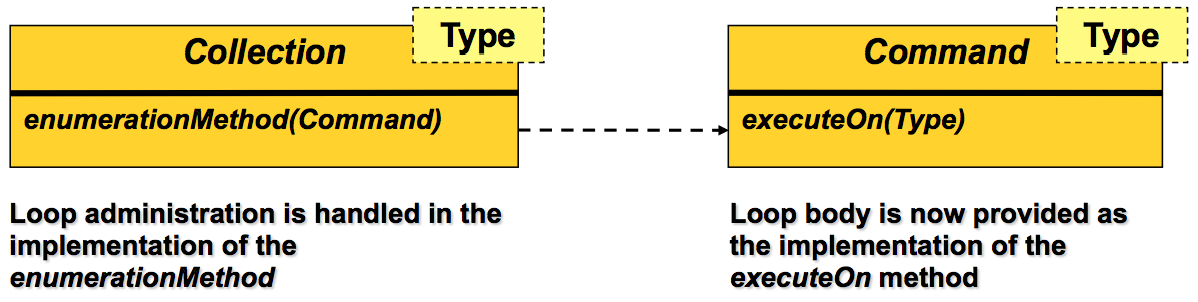
\includegraphics[width=0.9\textwidth]{content/advancedPatterns/enumerationmethod.png}
	\caption{Enumeration Method}
\end{figure}

\textbf{Vorteile}

\begin{itemize}
	\item Client ist nicht für die Verwaltung eines Iterators zuständig
	\item Synchronisation kann für die gesamte Traversierung gewährleistet werden, statt nur pro Zugriff
\end{itemize}

\textbf{Nachteile}

\begin{itemize}
	\item Führt zum Teil zu unnötig viel Code und Verschmutzung des Namespaces da viele Command Objekte benötigt werden
	\item Kann u.U. zur Verwirrung führen; ``zu abstrakt''
\end{itemize}


\section{Methods for States / Collections for States}

\textbf{Methods for States}

Stelle jeden Zustand als Tabelle von Methoden oder Funktionen dar, die über diese Tabelle aufgerufen werden.

\textbf{Collections for States}

Gruppiere Objekte im selben Zustand in Collections sodass der State durch dazugehörigkeit zu einer Collection repräsentiert wird.

